\documentclass{beamer}
\usetheme[pageofpages=de,% String used between the current page and the
                         % total page count.
          bullet=circle,% Use circles instead of squares for bullets.
          titleline=true,% Show a line below the frame title.
          alternativetitlepage=true,% Use the fancy title page.
          titlepagelogo=../img/fse_ministerio_ancho_texto.png%,% Logo for the first page.
	  %watermark=junta_girado,
          %watermarkheight=75px,% Height of the watermark.
          %watermarkheightmult=4,% The watermark image is 4 times bigger
                                % than watermarkheight.
          ]{Torino}

\usepackage[spanish]{babel} % Para separar correctamente las palabras
\usepackage[utf8]{inputenc} % Este paquete permite poner acentos y eñes usando codificación utf-8

\usepackage{color}
\usepackage{listings}

\author{
\small{IES Gonzalo Nazareno}\\
\tiny{Dos Hermanas (Sevilla)}\\
\small{IES Los Albares}\\
\tiny{Cieza (Murcia)}\\
\small{IES La Campiña}\\
\tiny{Arahal (Sevilla)}\\
\small{IES Ingeniero de la Cierva}\\
\tiny{Murcia}\\
\vspace{.5cm}

\includegraphics[width=0.2\textwidth]{cc_by_sa.png}}
\title{Introducción a OpenStack}
\institute{Proyecto de Innovación\\ {\color{white} .\\} \emph{Implantación y
    puesta a punto de la infraestructura de un cloud computing privado para el
    despliegue de servicios en la nube}}  


\lstset{basicstyle=\small,
aboveskip=5pt,
basicstyle=\tiny\ttfamily,
belowskip=5pt
}

\begin{document}
\setlength{\parskip}{.2cm}

\begin{frame}[t,plain]
\titlepage
\end{frame}

\begin{frame}
  \frametitle{Cloud Computing}
  Según la wikipedia:\par
  ``La computación en la nube, concepto conocido también bajo los términos
  servicios en la nube, informática en la nube, nube de cómputo o nube de
  conceptos, del inglés cloud computing, es un paradigma que permite ofrecer
  servicios de computación a través de Internet.''
\end{frame}

\begin{frame}
  \frametitle{Cloud Computing. Capas}
  Tradicionalmente se definen tres capas:
  \begin{description}
  \item[Software as a Service (SaaS)] Aplicación completa ofrecida
    como servicio en la nube (Servicios de Google, Salesforce.com, Microsoft
    Office 365, \ldots)
  \item[Platform as a Service (PaaS)] Aplicación completa para el
    desarrollo ofrecida como servicio en la nube (Google App Engine,
    Windows Azure, RedHat OpenShift, \ldots)
  \item[Infrastructure as a Service (IaaS)] Almacenamiento (también
    denominado \textit{Storage as a Service}) y capacidades de cómputo
    (máquinas completas) ofrecida como servicio en la nube.
  \end{description}
\end{frame}

\begin{frame}
  \frametitle{Cloud Computing. Tipos}
  \begin{description}
  \item[Público] Una empresa ofrece IaaS a terceros, encargándose de
    toda la gestión del Cloud. El caso más conocido es Amazon Elastic
    Compute Cloud (EC2).
  \item[Privado] Una organización configura sus propios recursos como
    IaaS para tener más flexibilidad y control total sobre sus
    recursos.
  \item[Híbrido] Algunos servicios se gestionan en el cloud privado y
    otros se transfieren a uno público, normalmente utilizan una API
    común que permita una buena integración.
  \end{description}
\end{frame}

\begin{frame}
  \frametitle{Inicios de OpenStack}
  \begin{tabular}[b]{cl}
    
\includegraphics[width=.2\textwidth]{../img/rackspace.jpg}&
    \parbox{0.75\textwidth}{
      \begin{itemize}
      \item Cloud propio desde 2005
        \begin{itemize}
        \item Cloud servers (IaaS)
        \item Cloud files (StaaS)
        \end{itemize}
      \item Este software cambia a licencia libre en Abril 2010
      \end{itemize}}\\
    \hline
    
\includegraphics[width=.1\textwidth]{../img/nasa.png}&
    \parbox{.75\textwidth}{
      \begin{itemize}
      \item Comienza a utilizar Eucalyptus, pero lo descarta por no ser
        completamente libre (es ``open core'')
      \item Crea el software para IaaS Nebula
      \item Nebula cambia a licencia libre en Mayo 2010
      \end{itemize}}\\
    \hline
    
\includegraphics[width=.1\textwidth]{../img/openstack.jpg}&
    \parbox{.75\textwidth}{
      \begin{itemize}
      \item Nasa y Rackspace lo inician en Junio de 2010
      \item Dos componentes principales:
        \begin{itemize}
        \item OpenStack Compute (nova), deriva de Nebula
        \item OpenStack Object Store (swift), deriva de cloud files
        \end{itemize}
      \end{itemize}}\\
  \end{tabular}
\end{frame}

\begin{frame}
  \frametitle{Objetivo de OpenStack}
  \begin{center}
    ``Crear una plataforma en software libre para cloud computing que cumpla con
    las necesidades de los proveedores de nubes públicas y privadas,
    independientemente de su tamaño, que sea fácil de implementar y masivamente
    escalable.''
  \end{center}
\end{frame}

\begin{frame}
  \frametitle{Principios fundacionales de OpenStack}
  \begin{itemize}
  \item Licencia Apache 2.0, no existe versión ``enterprise''
  \item Proceso de diseño abierto
  \item Repositorios públicos de código fuente
  \item Todos los procesos de desarrollo deben estar documentados y ser
    transparentes
  \item Orientado para adoptar estándares abiertos
  \item Diseño modular que permite flexibilidad mediante el uso de APIs
  \end{itemize}
\end{frame}
\begin{frame}[fragile]
  \frametitle{OpenStack es libre y abierto}
  \begin{itemize}
  \item OpenStack es un proyecto con licencia libre (Apache)
  \item Diseño abierto:
    \begin{itemize}
    \item \url{http://blueprints.launchpad.net/openstack}
    \item \url{http://www.openstack.org/summit/san-diego-2012/}
    \end{itemize}
  \item Desarrollo abierto:
    \begin{itemize}
    \item \url{http://launchpad.net/openstack} y \url{http://github.com/openstack/}
    \item Lenguaje de programación Python
    \item \url{http://bugs.launchpad.net/openstack/}
    \end{itemize}
    \item Comunidad abierta:
      \begin{itemize}
      \item \url{http://www.openstack.org/community/}
      \item \url{http://www.openstack.org/foundation/companies/}
      \item \url{http://lists.openstack.org}
      \end{itemize}
    \item Comunidad + empresas
  \end{itemize}
\end{frame}

\begin{frame}
  \frametitle{Versiones de OpenStack}
  \begin{itemize}
  \item Proyecto muy nuevo, pero con un fuerte ritmo de desarrollo
    \begin{description}
    \item[Austin] 21 Octubre 2010
    \item[Bexar] 3 Febrero 2011
    \item[Cactus] 15 Abril 2011
    \item[Diablo] 22 Septiembre 2011 (Publicación semestral)
    \item[Essex] 5 Abril 2012
    \item[Folsom] 27 Septiembre 2012
    \item[Grizzly] Previsto 4 Abril 2013
    \end{description}
  \item Está previsto que se publiquen dos versiones al año
  \item Hasta ahora cada versión incluye importantes modificaciones respecto a
    la anterior
  \item Essex ha sido la primera versión ``completa''
  \item Desde Cactus, el ritmo de publicación se acopla al de Ubuntu
  \end{itemize}
\end{frame}

\begin{frame}[fragile]
  \frametitle{OpenStack Essex (2012.1)}
  \begin{itemize}
  \item ¿Por qué es importante Essex?
    \begin{itemize}
    \item Primera versión completa de OpenStack para usar en producción
    \item Presente en Ubuntu 12.04 LTS. La próxima versión LTS será en 2014
    \item Presente en Debian Wheezy (próxima estable). Debian wheezy soportará
      OpenStack Folsom en backport
    \end{itemize}
  \item Componentes de OpenStack Essex:
    \begin{itemize}
    \item OpenStack Compute (nova)
    \item OpenStack Object Store (swift)
    \item OpenStack Image (glance)
    \item OpenStack Identity (keystone) $\leftarrow$ Nuevo en Essex
    \item OpenStack Dashboard (horizon) $\leftarrow$ Nuevo en Essex
    \end{itemize}
  \end{itemize}
  \url{http://wiki.openstack.org/ReleaseNotes/Essex}
\end{frame}

\begin{frame}
  \frametitle{OpenStack Folsom (2012.2)}
  \begin{itemize}
  \item OpenStack tiene un ritmo de publicación semestral, difícil de incluir en
    la publicación de distribuciones ``estables''. Ubuntu LTS o Debian se
    publican cada dos años.
  \item Incluye mejoras en bastantes componentes de OpenStack
  \item Incluido en Ubuntu 12.10
  \item Se incluirá en Debian Wheezy mediante backport (repositorio extra menos
    estable)
  \item Las principales novedades son la aparición de dos nuevos componentes
    principales:
    \begin{itemize}
    \item OpenStack Network Service (Quantum)
    \item OpenStack Block Storage (Cinder)
    \end{itemize}
  \end{itemize}
  \url{http://wiki.openstack.org/ReleaseNotes/Folsom}
\end{frame}

\begin{frame}
  \frametitle{¿Es OpenStack una buena opción?}
  \begin{itemize}
  \item A pesar de ser un proyecto muy nuevo, tiene un ritmo de desarrollo muy
    fuerte
  \item Cuenta con la mayor comunidad de desarrolladores dentro de los proyectos
    de software libre para cloud computing ($\sim$200 en Essex)
  \item Más de 100 empresas participan en el desarrollo en diferente medida
  \end{itemize}  
  \begin{columns}
    \hspace{.01cm}
    \column{.35\textwidth}
    \begin{itemize}
    \item Esto es consecuencia de la orientación libre y abierta del proyecto
    \item Has oído hablar de OpenStack con motivo, esto no es vaporware
    \end{itemize}
    \column{.6\textwidth}
    Google Trends:
    \begin{center}
      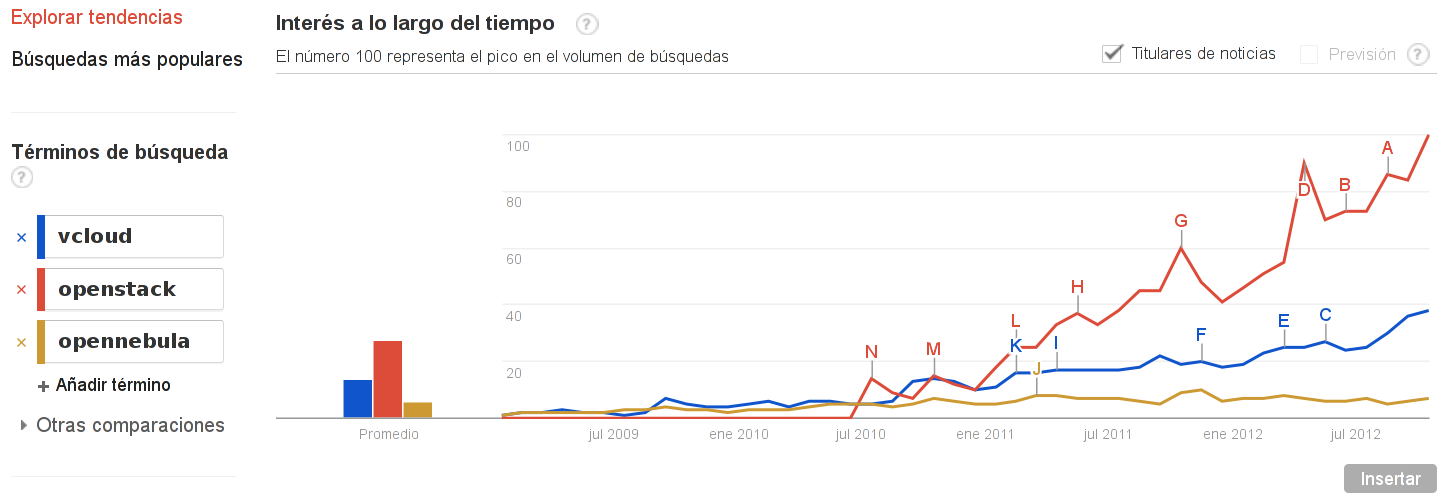
\includegraphics[width=\textwidth]{../img/google_trends.png}
    \end{center}
  \end{columns}
\end{frame}

\begin{frame}
  \frametitle{Servicios de OpenStack nova}
  \begin{itemize}
  \item Nova es el componente principal de OpenStack y está compuesto por varios
    servicios independientes:
    \begin{description}
    \item[nova-api] Encargado de aceptar las peticiones de los usuarios o del
      resto de componentes de OpenStack mediante una API RESTful
    \item[nova-scheduler] Encargado de planificar la ejecución de las instancias
      en los diferentes nodos del cloud
    \item[nova-compute] Encargado de ejecutar una instancia sobre un hipervisor
    \item[nova-network] Encargado de la comunicación de la instancia con el
      exterior
    \item[nova-volume] Encargado de gestionar los volúmenes asociados a las
      instancias
    \end{description}
  \item Los componentes de nova se comunican entre sí mediante AMQP
  \end{itemize}
\end{frame}

\begin{frame}
  \frametitle{Funcionamiento típico de OpenStack}
  \begin{itemize}
  \item Un usuario interactúa con la API de nova (bien directamente o
    indirectamente a través de horizon) para ejecutar una instancia.
  \item nova-api le pedirá que se autentique previamente con keystone
  \item Una vez autenticado le mostrará las imágenes disponibles en glance
  \item Cuando seleccione una imagen y unas características para la instancia,
    se enviará a nova-scheduler la petición
  \item Nova-scheduler determinará en que nodo debe ejecutarse la instancia
  \item Nova-compute del nodo seleccionado se encargará de ejecutar la instancia
    sobre el hipervisor que disponga
  \item Nova-network realizará las configuraciones necesarias en la red
  \item Nova-volume se encargará de gestionar en su caso los volúmenes asociados
    a la instancia
  \end{itemize}
\end{frame}

\begin{frame}
  \frametitle{Funcionamiento de OpenStack}
  \begin{center}
    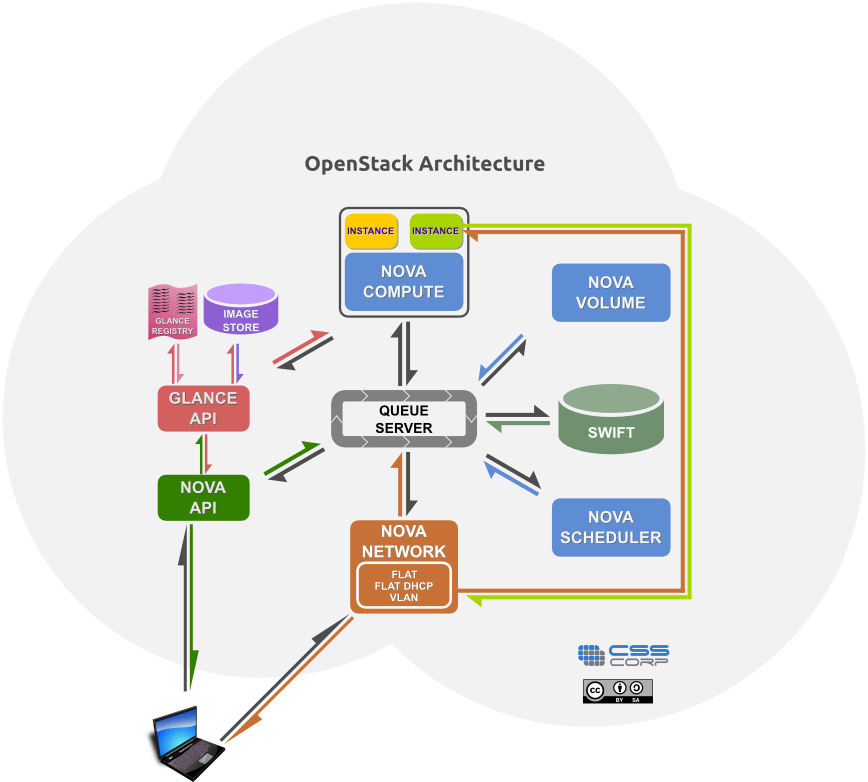
\includegraphics[height=.75\textheight]{../img/Archhtml.png}
  \end{center}
\end{frame}

\begin{frame}
  \frametitle{Instalación de componentes de OpenStack }
  \begin{itemize}
  \item Dependiendo del número de equipos del cloud y la configuración de red,
    se instalarán en cada nodo diferentes componentes, p. ej.:
  \end{itemize}
  \begin{center}
    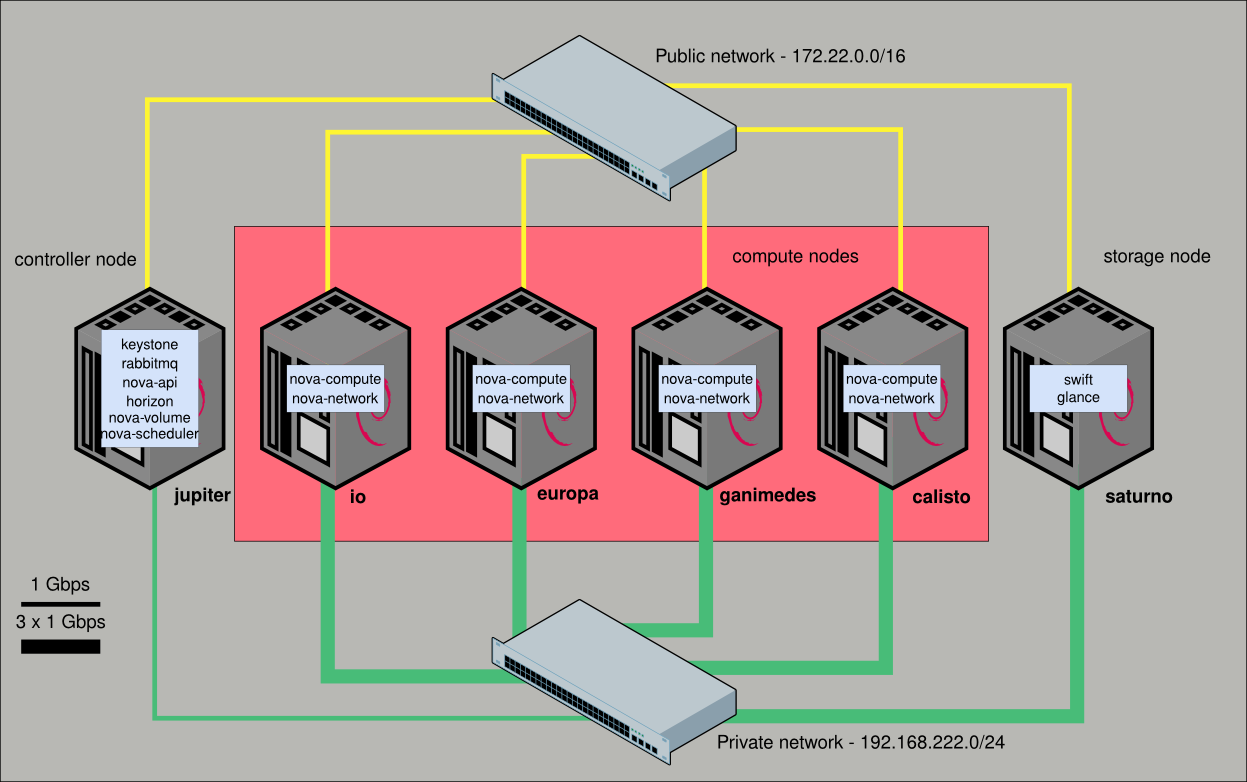
\includegraphics[width=.8\textwidth]{../img/esquema_red_iesgn}    
  \end{center}
\end{frame}

\begin{frame}[fragile]
  \frametitle{APIs}
  \begin{itemize}
  \item Cada componente de OpenStack ofrecen una API RESTful
  \item Las APIs se pueden utilizar con XML o JSON (por defecto JSON)
  \item Esto hace OpenStack extensible y adaptable a cada entorno
  \end{itemize}
  \begin{center}
  \begin{lstlisting}
$ nova --debug list
connect: (172.22.222.1, 5000)
send: 'POST /v2.0/tokens HTTP/1.1\r\nHost: 172.22.222.1:5000\r\nContent-Length:124
\r\ncontent-type: application/json\r\naccept-encoding: gzip, deflate\r\naccept: ap
plication/json\r\nuser-agent: python-novaclient\r\n\r\n{"auth": {"tenantName": "te
st", "passwordCredentials": {"username": "user", "password": "testpass"}}}'
reply: 'HTTP/1.1 200 OK\r\n'
connect: (172.22.222.1, 8774)
send: u'GET /v2/aaaaaaaa5894473c8a98f89a895c6b2c/servers/detail HTTP/1.1\r\nHost: 
172.22.222.1:8774\r\nx-auth-project-id: test\r\nx-auth-token: e9233fef4ce34ee49f7d
b1aaaaaaa13f\r\naccept-encoding: gzip, deflate\r\naccept: application/json\r\nuser
-agent: python-novaclient\r\n\r\n'
reply: 'HTTP/1.1 200 OK\r\n'
+--------------------------------------+--------+---------------+----------------+
|                  ID                  |  Name  |     Status    |    Networks    |
+--------------------------------------+--------+---------------+----------------+
| b1724bd0-34f4-4bf1-9444-110eb3531602 | demo9  | VERIFY_RESIZE | vlan5=10.0.5.6 |
| e82814aa-fb1d-4c29-81ab-c39f99184413 | demo10 | ACTIVE        | vlan5=10.0.5.3 |
+--------------------------------------+--------+---------------+----------------+
  \end{lstlisting}
\end{center}
\end{frame}

\end{document}
